\documentclass[conference]{IEEEtran}
\IEEEoverrideCommandLockouts
\usepackage{cite}
\usepackage{amsmath,amssymb,amsfonts}
\usepackage{graphicx}
\usepackage{textcomp}
\usepackage{xcolor}
\usepackage{booktabs}
\usepackage{url}
\usepackage{siunitx}
\sisetup{detect-all, per-mode=symbol}

% AUTO-GENERATED by scripts/plot_results.py --emit-macros. Do not edit by hand.
% source: eval_on.npz  checkpoint iter 4500  (2026-08-02T00:11:59)
\newcommand{\PLACEHOLDER}{\textcolor{red}{\textbf{??}}}

\newcommand{\RESnepisodes}{727}
\newcommand{\RESnepisodesAbl}{704}
\newcommand{\RESckpt}{4500}
\newcommand{\RESfracintol}{67\%}
\newcommand{\RESablsuccess}{0.0\%}

\newcommand{\RESsuccess}{48.4\%}
\newcommand{\RESsuccessCI}{[44.8, 52.0]}
\newcommand{\RESreachrate}{89.8\%}
\newcommand{\RESposonly}{96.8\%}
\newcommand{\RESorionly}{93.8\%}

\newcommand{\RESdfinal}{20.1}
\newcommand{\RESthetafinal}{14.5}
\newcommand{\REStreach}{0.94}
\newcommand{\REStsuccess}{2.01}

\newcommand{\RESjerkOn}{654}
\newcommand{\RESjerkOff}{364170}
\newcommand{\RESjerkRatio}{557.2$\times$}
\newcommand{\RESvelOn}{4.10}
\newcommand{\RESvelOff}{42.49}
\newcommand{\REScmdvelOn}{2.00\,rad/s}
\newcommand{\REScmdaccOn}{15.0\,rad/s$^2$}


\newcommand{\vect}[1]{\mathbf{#1}}

\begin{document}

\title{A Domain-Randomized Isaac Lab Environment for Orchard Manipulation with the Unitree G1: Learned, Optimization-Based and Hybrid Pre-Grasp Reaching
\thanks{Identify applicable funding agency here. If none, delete this.}
}

\author{\IEEEauthorblockN{1\textsuperscript{st} Pablo Kevin Pereira}
\IEEEauthorblockA{\textit{Mechatronics Engineering} \\
\textit{Universidad Tecnológica (UTEC)}\\
Fray Bentos, Uruguay \\
pablo.pereira.p@estudiantes.utec.edu.uy}
\and
\IEEEauthorblockN{2\textsuperscript{nd} Lucas Baldezzari}
\IEEEauthorblockA{\textit{Biomedical Engineering} \\
\textit{Universidad Tecnológica (UTEC)}\\
Fray Bentos, Uruguay\\
lucas.baldezzari@utec.edu.uy}
\and
\IEEEauthorblockN{3\textsuperscript{rd} Fernando Auat Cheein}
\IEEEauthorblockA{\textit{Engineering Department} \\
\textit{Harper Adams University}\\
Newport, Shropshire TF10 8NB \\
FAuat@harper-adams.ac.uk}
\and
\IEEEauthorblockN{4\textsuperscript{th} Nestor Nahuel Deniz}
\IEEEauthorblockA{\textit{Engineering Department} \\
\textit{Harper Adams University}\\
Newport, Shropshire TF10 8NB \\
ndeniz@harper-adams.ac.uk}
}

\maketitle

\begin{abstract}
Robotic apple harvesting requires the hand to reach a specific point relative to
the fruit, in a specific orientation, before any grasp can succeed. We present an
open Isaac Lab environment posing this \emph{pre-grasp} problem for the Unitree
G1 humanoid with Dex3 hands, in which a procedurally randomized tree is rebuilt
every episode and the fruit is sampled directly in the shoulder's polar
coordinates so targets are geometrically varied but kinematically meaningful.
Motion smoothness is structural rather than learned: a rate-limited action term
caps commanded joint velocity and acceleration for any policy output whatsoever.
Within one interface we compare three controllers---a PPO policy, a CasADi/IPOPT
inverse-kinematics solver, and a hybrid that hands off from the first to the
second. Over \RESnepisodes{} randomized episodes the policy is fast
(\RLforward{}\,ms per decision) and reaches the position tolerance on
\RESposonly{} of episodes but cannot hold orientation, succeeding on
\RESsuccess{}; the solver is exact but costs \CASsolveMed{}\,ms with a
\CASsolveMax{}\,ms worst case; the hybrid reaches \HYBsuccess{} at
\HYBcompute{}\,ms per episode. We also report a negative result we consider the
most transferable: a densely shaped reward with mis-specified grasp geometry
converges confidently---position terms saturate, action noise collapses---while
task success never leaves zero, and no training curve reveals it.
\end{abstract}

\begin{IEEEkeywords}
reinforcement learning, humanoid manipulation, agricultural robotics, inverse
kinematics, simulation environments
\end{IEEEkeywords}

% ═══════════════════════════════════════════════════════════════
\section{Introduction}
% ═══════════════════════════════════════════════════════════════

Harvesting robots for high-value crops have been studied for decades, and the
recurring conclusion is that the unstructured canopy---not the gripper, not the
picking motion---limits field
performance~\cite{zhang2022apple,jangali2024endeffector}. Purpose-built apple
harvesters reach the fruit with task-specific manipulators and hand-engineered
approach trajectories~\cite{zhang2022apple,zhang2024apple}. A general-purpose
humanoid with a multi-fingered hand is an attractive alternative, and
reinforcement learning has produced dexterous behaviour that transfers to
hardware~\cite{handa2023dextreme,he2025hover}; but such a platform inherits none
of that task-specific engineering, so the approach pose must be learned or
planned.

GPU-parallel simulation makes learning it tractable~\cite{mittal2023orbit}, and
learned loco-manipulation is now routine on legged and humanoid
platforms~\cite{fu2026demohlm,liu2026mlm}, including in
agriculture~\cite{ma2026weeding}. The reference environments published for the
Unitree family, however, target locomotion and motion imitation:
\texttt{unitree\_rl\_lab} registers velocity tracking for Go2, H1 and G1 plus
motion-mimic tasks~\cite{unitree_rl_lab}, and manipulation support for the G1
with Dex3 hands exists as teleoperation and data
collection~\cite{unitree_sim_isaaclab}, not as a learning task. To our knowledge
no open Isaac Lab environment poses orchard manipulation for this platform.

% Floats to the top of column 2 on page 1.
\begin{figure}[!t]
\centering

\includegraphics[width=\columnwidth]{figures/scene_g1_reach.png}
\caption{The Unitree G1 with Dex3 hands at a pre-grasp pose beneath an apple in
the randomized environment. The hand approaches from below with the palm normal
aligned to gravity---the configuration a subsequent grasp requires. Trunk
height, branch length and yaw, and fruit radius and mass are redrawn per
environment.}
\label{fig:hero}
\end{figure}

We contribute (i) a randomized orchard manipulation environment for the G1
(Fig.~\ref{fig:hero}) built from procedural primitives, so canopy geometry is a
randomization axis rather than a fixed asset; (ii) an action interface that
bounds commanded velocity and acceleration structurally, with a minimum-jerk
supervisor for arrival; (iii) a task whose success criterion is a \emph{held}
pose, as a grasp actually requires; and (iv) a three-way comparison---learned,
optimization-based, and hybrid---within that single interface, with an explicit
account of how each fails.

% ═══════════════════════════════════════════════════════════════
\section{Environment and Task}
\label{sec:env}
% ═══════════════════════════════════════════════════════════════

The environment is a \texttt{ManagerBasedRLEnv} on Isaac
Lab~\cite{mittal2023orbit} (v2.3.2, Isaac Sim 4.5). Physics runs at
\SI{200}{\hertz} with decimation 4, giving \SI{50}{\hertz} control; episodes last
\SI{5}{\second} (250 steps) and 64 environments run in parallel. The robot is a
Unitree G1 29-DoF humanoid with Dex3 hands, converted to USD from the vendor
URDF~\cite{unitree_ros}. The pelvis is fixed---the task is manipulation, not
locomotion---and only the seven right-arm joints are actuated, through implicit
PD actuators at $k_p=100$, $k_d=10$.

\subsection{Procedural tree and inverse fruit placement}

The tree is not an imported asset but three primitives---a cuboid base, a
cylindrical trunk, a cylindrical branch---whose dimensions are drawn per
environment at $\pm20\%$ around nominal values (\SI{1.25}{\metre} trunk,
\SI{0.50}{\metre} branch, $140^\circ$ yaw) and written to the USD stage before
simulation starts. Fruit radius and mass are likewise randomized around
\SI{0.04}{\metre} and \SI{0.15}{\kilo\gram}. Building the canopy from
parameterized primitives rather than a fixed mesh makes its geometry a
randomization axis~\cite{shakerimov2023domainrand,ahsen2025domainrand}, so a
policy cannot memorize one tree.

Placement runs opposite to the visual hierarchy. Each reset samples the
\emph{fruit} in the right shoulder's polar coordinates---azimuth
$\psi\sim\mathcal{U}(-77.5^\circ,-12.5^\circ)$ and a horizontal radius chosen so
the 3-D shoulder-to-target distance lies in $[r_{\min},r_{\max}] =
[0.30,0.62]$\,m---then solves the trunk pose backwards so the branch tip meets
it. This inversion matters: sampling tree pose and branch geometry independently,
as an earlier version did, routinely placed the fruit outside the workspace, and
a policy cannot learn reaching from unreachable targets.

In this reach-only phase the fruit is \emph{kinematic}: a dynamic fruit on a
PhysX fixed joint was attempted first, but the joints failed to replicate
per-environment and fruit collapsed to one shared height. Reaching only requires
the fruit to stay put, so we kinematize it and defer the dynamic body to the
grasp phase---at the cost of inactive contact rewards, so the Dex3 joints leave
the action space.

\subsection{Task definition}

A grasp needs the hand positioned \emph{and} oriented; reaching the right point
with the palm facing sideways is useless. The task is defined by the distance
$d$ from a palm-fixed grasp reference point to a target $\delta_z =
\SI{0.068}{\metre}$ below the fruit centre, and the angle $\theta$ between the
palm normal and world $+z$. Both are measured from points determined empirically
rather than read off the URDF: the palm link origin lies near the wrist, some
\SI{0.08}{\metre} short of the contact area along its local $+x$, and the palm
normal is a specific local axis identified by probing each axis's world-frame
image. Success is a \emph{termination}: the episode ends once
$d<\SI{40}{\milli\metre}$ and $\theta<0.30$\,rad have held continuously for
\SI{0.5}{\second}. Requiring a hold rather than an instant of proximity is what
distinguishes a settled pre-grasp state from a fly-through.

\subsection{Rate-limited action interface}
\label{sec:action}

All three controllers drive the arm through one interface. The action is a 7-D
joint position target mapped as $\tilde{q}_t = \mathrm{clip}(0.5\,\vect{a}_t +
q_{\text{def}},\pm3)$. Applying $\tilde{q}_t$ directly---Isaac Lab's stock
behaviour---lets a controller jump several radians every
\SI{20}{\milli\second}, saturating the actuator into bang-bang acceleration at
the control rate. We therefore treat $\tilde{q}_t$ as a \emph{desired} target and
integrate a rate-limited command,
\begin{align}
v^{\text{des}}_t &= (\tilde{q}_t - q^{\text{cmd}}_{t-1})/\Delta t, \nonumber\\
v_t &= \mathrm{clip}\big(\mathrm{clip}(v^{\text{des}}_t, \pm v_{\max}),\;
        v_{t-1} \pm a_{\max}\Delta t\big), \label{eq:ratelimit}\\
q^{\text{cmd}}_t &= q^{\text{cmd}}_{t-1} + v_t \Delta t, \nonumber
\end{align}
with $v_{\max}=\SI{2.0}{\radian\per\second}$ and
$a_{\max}=\SI{15}{\radian\per\second\squared}$. The bound holds for any output
whatsoever, so commanded jerk is capped at $2a_{\max}/\Delta t =
\SI{1500}{\radian\per\second\cubed}$. Measured over \RESnepisodes{} episodes the
commanded velocity and acceleration reach exactly \REScmdvelOn{} and
\REScmdaccOn{} and never exceed them. This is load-bearing rather than cosmetic:
re-running the trained policy with the limits removed raises jerk RMS by
\RESjerkRatio{} and drops success to \RESablsuccess{}---the policy learns to emit
targets that are \emph{integrated}, and removing the integrator changes the
plant.

A second mechanism handles arrival. A controller rewarded densely for proximity
has no incentive to stop moving beside an object it can damage, and outside
simulation there is no episode boundary to hide it. A supervisor therefore
monitors palm-to-fruit distance and, once it stays below a threshold for a dwell
time, brings the arm to rest on a quintic minimum-jerk profile solved for
$q(0)=q_0,\dot q(0)=v_0,\ddot q(0)=0$ and $q(T)=q_1,\dot q(T)=\ddot q(T)=0$, with
the stopping point derived as $q_1=q_0+v_0T/2$. Matching $\dot q(0)=v_0$ is the
point: zeroing the targets on arrival is a velocity discontinuity, exactly the
jerk the design avoids.

\subsection{Reward and training}
\label{sec:reward}

The reward has fourteen terms: a potential-based progress term $d_{t-1}-d_t$
($+10$) for dense gradient at any distance; two Gaussians in $d$ at
$\sigma=0.25$ and $0.04$ ($+1$, $+4$) giving a coarse basin and a sharp peak; a
per-step hold bonus ($+3$) and terminal success bonus ($+75$) rewarding staying
rather than arriving; a distance-gated palm-up term ($+1.5$) for orientation; and
regularizers on action rate and jerk, joint velocity, near-goal braking, joint
limits, and home posture---the last weighted onto shoulder and elbow but not the
wrist, which must stay free for orientation.

We train with PPO~\cite{schulman2017ppo} in the massively parallel configuration
established for legged locomotion~\cite{rudin2022walk}: separate
$128$--$128$--$64$ ELU actor and critic over a 28-D observation (joint positions
and velocities, palm-to-fruit vector, palm quaternion relative to torso, previous
action), $64$ steps $\times$ $64$ environments per iteration, five epochs over
four minibatches, adaptive learning rate targeting $\mathrm{KL}=0.01$,
$\gamma=0.99$, $\lambda=0.95$. A $3000$-iteration run is $12.3\times10^6$ steps
and takes \SI{78}{\minute} on a laptop RTX~4060; the reported policy continues to
\RESckpt{} iterations.

% ═══════════════════════════════════════════════════════════════
\section{Three Controllers, One Interface}
\label{sec:controllers}
% ═══════════════════════════════════════════════════════════════

Two alternatives publish joint targets through the same rate-limited term and
arrival supervisor, so all three are interchangeable and differ only in how the
target is produced. The \textbf{CasADi controller} builds the arm's forward
kinematics symbolically from the URDF and solves, every tick, a small nonlinear
program in CasADi~\cite{andersson2019casadi} with IPOPT that penalises
grasp-point position error, palm-normal misalignment and deviation from the
previous solution subject to joint limits, warm-started from the last solve---
mirroring the optimization-based control standard for legged and mobile
manipulators~\cite{molnar2026wbid,rahman2026locoreview}. The \textbf{hybrid} runs
the policy until the palm is within \SI{10}{\centi\metre} of the fruit or
\SI{2.5}{\second} elapse, then hands off to the solver: the policy is cheap and
generalizes but plateaus a few centimetres short, precisely the regime an exact
solve handles well, while running IPOPT throughout would spend its per-tick cost
on the easy far field.

% ═══════════════════════════════════════════════════════════════
\section{Results}
\label{sec:results}
% ═══════════════════════════════════════════════════════════════

We evaluate the deterministic policy over \RESnepisodes{} randomized episodes.
The solver and hybrid are scored on the \emph{same} targets: the solver on each
recorded target directly, the hybrid by replaying its switching logic over the
recorded rollouts and running the real IPOPT solve from the arm's state at
handoff. Solver residuals are therefore open-loop kinematic error---whether a
configuration exists and is found---while the policy's are realised after
\SI{5}{\second} of physics including the hold.

\begin{table}[t]
\centering
\caption{Three controllers on identical targets. Compute is per decision for the
policy and solver, per episode for the hybrid.}
\label{tab:compare}
\small
\begin{tabular}{lrrr}
\toprule
& Policy & CasADi & Hybrid \\
\midrule
Satisfies both tolerances & \RESsuccess{} & \CASfeasible{} & \HYBsuccess{} \\
\quad position & \RESposonly{} & \CASposfeasible{} & \HYBpos{} \\
\quad orientation & \RESorionly{} & \CASorifeasible{} & \HYBori{} \\
\midrule
Position error, median [mm] & \RESdfinal{} & \CASposMed{} & \HYBdfinal{} \\
Orientation error, med.\ [deg] & \RESthetafinal{} & \CASoriMed{} & \HYBtheta{} \\
Time to settle [s] & \REStsuccess{} & --- & \HYBttotal{} \\
\midrule
Compute, median [ms] & \RLforward{} & \CASsolveMed{} & \HYBcompute{} \\
\quad worst case [ms] & --- & \CASsolveMax{} & --- \\
\bottomrule
\end{tabular}
\end{table}

\begin{figure}[t]
\centering
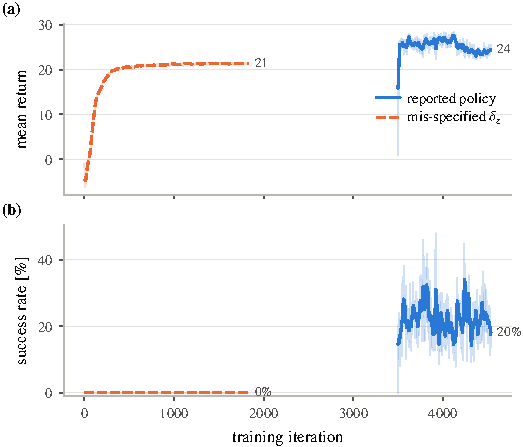
\includegraphics[width=\columnwidth]{figures/fig1_training.pdf}
\caption{Training curves for the reported policy and an earlier configuration
with mis-specified grasp geometry. Return (a) rises in both; task success (b) is
flat at zero throughout the mis-specified run, whose position reward is in fact
\emph{higher}. The reported policy resumed from a checkpoint, so its log starts
at iteration 3500. The runs also differ in reach envelope, so this is
illustrative rather than a single-variable ablation.}
\label{fig:training}
\end{figure}

\subsection{A confidently converged, entirely unsuccessful policy}
\label{sec:negative}

Fig.~\ref{fig:training} contrasts the reported run with an earlier configuration
whose grasp offset was $\delta_z=\SI{0.164}{\metre}$, more than twice the
reported \SI{0.068}{\metre}, inside a tighter envelope. By the usual signals it
converged well: return climbed to within \SI{20}{\percent} of the working run's,
the fine-reach reward \emph{saturated higher} ($3.40$ against $2.72$ of a maximum
$4.0$), and action-noise standard deviation collapsed from $0.50$ to $0.025$.
Its success rate was exactly zero on all $1830$ iterations.

Both runs share the same palm-normal axis, so this is a geometric error, not a
frame-convention one: a grasp point \SI{0.164}{\metre} below the fruit sits low
and close to the torso, where the elbow folds inward and little wrist authority
remains for orientation, making the two objectives jointly unsatisfiable. The
point is the \emph{observability}: nothing in the return, loss or entropy curves
indicates it---the entropy collapse resembles healthy convergence---and only the
success termination, defined against the task rather than any reward term,
reveals it. A shaped-reward manipulation task should carry at least one binary,
geometrically defined success signal that no reward term contributes to, purely
as an instrument.

\subsection{How the three controllers fail differently}

\begin{figure*}[t]
\centering
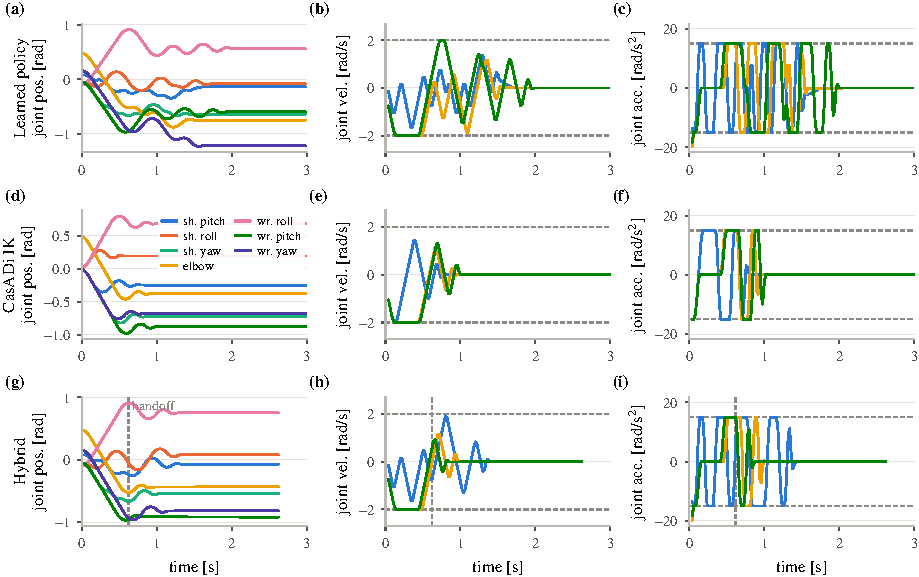
\includegraphics[width=\textwidth]{figures/fig_compare.pdf}
\caption{Commanded joint trajectories and Cartesian end-effector paths for one
target under the policy \textbf{(a--d)}, the CasADi solver \textbf{(e--h)}, and
the hybrid \textbf{(i--l)}. All pass through the same rate-limited interface and
all Cartesian paths use the same forward kinematics, so rows differ only in what
generates the target. Dashed rules are $v_{\max}$ and $a_{\max}$; the vertical
rule in the bottom row marks the handoff. The policy rides both bounds
continuously and never settles; the solver converges by
$\approx\SI{0.9}{\second}$ and then commands exactly zero; the hybrid inherits
the policy's fast approach and the solver's settling.}
\label{fig:compare}
\end{figure*}

Table~\ref{tab:compare} and Fig.~\ref{fig:compare} give the comparison. Each
criterion is separately near-solved by the policy---position tolerance met at
some point in \RESposonly{} of episodes, orientation in \RESorionly{}---yet
jointly only \RESsuccess{}. Fig.~\ref{fig:eval} shows why: position error
collapses below tolerance within \SI{1}{\second} and stays, but orientation error
\emph{oscillates around} its tolerance, crossing repeatedly rather than settling
beneath it. Episodes that entered the tolerance left it a median of three times
and spent only \RESfracintol{} of post-entry steps inside. Orientation is the
binding constraint and the failure mode is an unsettled hover, not a miss---
visible in Fig.~\ref{fig:compare}(a--d) as saturation of both bounds for the
entire episode.

The solver inverts this. It satisfies orientation on \CASorifeasible{} of targets
but position on only \CASposfeasible{}: with these cost weights it protects
orientation and yields position when they conflict. Where a solution exists it is
essentially exact (\CASposMed{}\,mm) and it settles---after
$\approx\SI{0.9}{\second}$ its commanded velocity and acceleration are exactly
zero. Its cost is compute: \CASsolveMed{}\,ms median against the policy's
\RLforward{}\,ms, and a \CASsolveMax{}\,ms worst case, an order of magnitude
beyond the \SI{20}{\milli\second} control period. A classical controller that
occasionally misses its deadline needs an explicit fallback; a network with
constant cost does not.

The hybrid captures most of both. It reaches \HYBsuccess{}---matching the
solver's \CASfeasible{} and far above the policy's \RESsuccess{}---with median
orientation error \HYBtheta{}$^\circ$ against \RESthetafinal{}$^\circ$, because
the solver finishes the pose the policy could not hold. Its advantage over the
solver is cost, not accuracy: \HYBcompute{}\,ms per episode against roughly
\SI{1.5}{\second} if IPOPT ran for all 250 ticks, since the policy covers the
easy far field for the price of a forward pass. Smoothness does not suffer at
the handoff: jerk RMS is \HYBjerk{}\,rad/s$^3$, slightly \emph{below} the
policy's own \RESjerkOn{}, because the rate limiter lives in the environment
rather than the client and its buffers carry straight through the switch
(Fig.~\ref{fig:compare}(i--l)).

One tuning observation. Handoff occurs at a median \HYBhandoff{}\,s but only
\HYBbyprox{} of episodes hand off by proximity rather than timeout: the policy
frequently does not close to \SI{10}{\centi\metre} of raw palm-to-fruit distance
within \SI{2.5}{\second}, so the timeout is doing more of the work than intended.
A larger switch radius, or a switch on the policy's own stagnation rather than on
distance, is the obvious next step.

\subsection{Where this works, and where it does not}
\label{sec:limitations}

\begin{figure}[t]
\centering
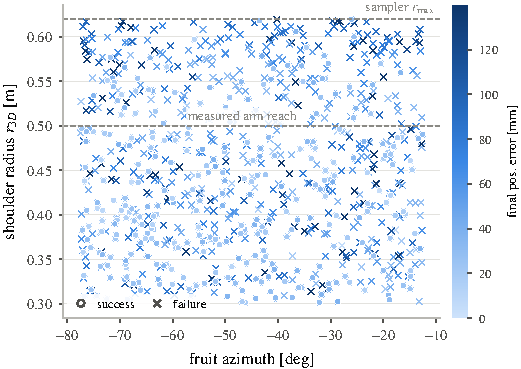
\includegraphics[width=\columnwidth]{figures/fig_eval.pdf}
\caption{\textbf{(a,b)} Position and orientation error across all episodes:
median with interquartile and $10$--$90$ bands, dashed rules at the tolerances.
\textbf{(c)} Outcome against where the fruit was sampled, in the randomizer's own
polar coordinates; colour encodes final position error. Above the measured
arm-reach rule almost everything fails.}
\label{fig:eval}
\end{figure}

Performance is reliable over the middle of the reach envelope and fails at both
ends for different reasons. \textbf{Near the body}, reaching requires folding the
elbow toward the torso. Self-collision is disabled in the articulation
configuration---enabling it on a 29-DoF humanoid is expensive and destabilizes
the solver---so nothing penalizes a configuration passing through the robot's own
body, and at small radii the policy produces them. Such episodes can be scored as
successes despite not being physically realizable.

\textbf{At long extension} the limit is kinematic. The shoulder-to-palm chain
measures about \SI{0.42}{\metre}, extended by the \SI{0.08}{\metre} palm offset,
for a ceiling near \SI{0.50}{\metre}---below the sampler's
$r_{\max}=\SI{0.62}{\metre}$. Fig.~\ref{fig:eval}c shows the consequence: above
the measured-reach rule almost every episode fails. The solver confirms this
independently, its residuals being strongly bimodal (\CASposMed{}\,mm median
against \CASposPninetyfive{}\,mm p95)---full model knowledge still cannot reach
roughly one target in five, because those targets are outside the workspace. That
ceiling belongs to the sampling envelope, not to any controller; we report
unfiltered numbers, so Table~\ref{tab:compare} understates performance on
feasible targets. Finally, the fruit is kinematic, so nothing here demonstrates
contact behaviour, and orientation accuracy is a claim about approach pose only,
not grasp stability.

% ═══════════════════════════════════════════════════════════════
\section{Conclusion and Future Work}
% ═══════════════════════════════════════════════════════════════

We presented an Isaac Lab environment posing orchard manipulation for the Unitree
G1 with Dex3 hands, and compared a learned policy, an optimization-based solver
and a hybrid within one bounded action interface. The learned policy is cheap and
generalizes but does not settle; the solver is exact and settles but is
expensive and occasionally misses its deadline; the hybrid recovers most of both
at a fraction of the solver's cost. Three design choices carried the weight:
sampling the fruit in the shoulder's coordinates so targets are kinematically
meaningful; enforcing smoothness structurally rather than through reward shaping;
and instrumenting the task with a success signal no reward term contributes to,
which is what made the failure of Sec.~\ref{sec:negative} visible at all.

The clearest next step is \textbf{tactile sensing in the palm}. Every controller
here decides it has arrived from a \emph{geometric} distance to an estimated
fruit centre, inheriting every error in fruit localisation, palm-offset
calibration and assumed fruit radius---all determined empirically, all liable to
drift. Contact is the physical event the task actually cares about, and a
palm-mounted tactile array reports it directly. We would \emph{replace} the
supervisor's geometric trigger with a tactile one rather than run both: a second
thread polling distance adds latency and another failure mode for a signal that
is strictly weaker evidence than contact itself, and the quintic stop needs only
a trigger instant, not a continuous distance. The same sensing then serves the
grasp phase, for which the contact sensors and Dex3 action term are already
present and need only the dynamic fruit body this phase defers.

Three further directions follow. Aligning the sampling envelope with the arm's
measured reach and enabling self-collision would remove both failure regions of
Sec.~\ref{sec:limitations}. The comparison suggests tighter integration than a
hard switch: a learned residual on top of the solver rather than a handoff
between them. And the head-camera variant would let a perception front-end of the
kind used for orchard fruit localisation~\cite{selvaraj2024segmentation} replace
the privileged fruit pose assumed throughout.

\section*{Acknowledgment}

The authors thank the Unitree Robotics team for publishing the G1 robot
description and the Isaac Lab reference environments this work builds on.

\bibliographystyle{IEEEtran}
\bibliography{refs}

\end{document}
